\documentclass[12pt, twocolumn]{article}
\usepackage[margin=3cm]{geometry}
\usepackage{listings}
\usepackage{graphicx}
\usepackage{float}
%\usepackage{tikz}
\usepackage[justification=centering]{caption}
%\usetikzlibrary{shapes.geometric,arrows}
%\renewcommand{\lstlistingname}{\textbf{Program}}
\newcommand{\sanper}{\textsc{sanper-1 elu} }
%setting up flowcharts
%\tikzstyle{startstop} = [rectangle, rounded corners, minimum width=3cm, minimum height = 1cm, text centered, draw=black, fill=red!30]

%\tikzstyle{process} = [rectangle, minimum width=3cm, minimum height = 1cm, text centered, text width = 3cm, draw=black, fill=orange!30]

%\tikzstyle{decision} = [diamond,  minimum width=1cm, minimum height = .5cm, text centered, text width = 2cm, draw=black, fill=green!30]

%\tikzstyle{arrow} = [thick, ->,>=stealth]

\begin{document}

\begin{titlepage}
	\begin{center}
		
		
		% Upper part of the page. The '~' is needed because \\
		% only works if a paragraph has started.
		\vfill
		
		\textsc{\LARGE Experiment 5: Memory Design Using Static Random Access Memory (RAM)}\\[1.5cm]
		
		\Large Adam Sumner\\[0.5cm]
		
		\Large Illinois Institute of Technology\\[0.5cm]
		
		\Large ECE 441-01\\[0.5cm]	
		% Author and supervisor
		\noindent
		\vfill
		\large \textbf{Lab Date:} March 3rd, 2015\hfill
		\large \textbf{Due Date:} March 31st, 2015
		% Bottom of the page
		
		
	\end{center}
\end{titlepage}

\section{Introduction}
The purpose of this experiment is to familiarize the user with the following devices and concepts:
\begin{itemize}
	\item Open Collector Devices
	\item Partial Decoding
	\item Static Random Access Memory (SRAM)
	\item The \sanper Block Select Lines
\end{itemize}

\section{Background}
\subsection{MC68000 Asynchronous Bus Interface}
The MC68000 has a 16-bit data bus, and byte accesses of memory locations are permitted from either an even or an odd address 
\subsection{Static RAM Devices}
Static Random Access Memory is a type of semiconductor memory that uses latching circuitry to store each bit. Its implementation is opposite of Dynamic Random Access Memory because when using DRAM, it must be periodically refreshed to hold on to data. SRAM does not require this type of ``maintenance." SRAM is volatile memory, so if power to the memory is no longer present, all data stored will be lost. The SRAM implemented in this lab is the MCM2114 Static RAM IC. It supplies 1K by 4-bits of memory. It supports 10 address lines, 4 data lines, a select input, and a R/$\overline{W}$ input.
\subsection{Open Collector Devices}
A standard TTL type device has two output transistors that form the output driver for the logic gate. The transistors are placed about each other, and the emitter of the top transistor is tied to the collector of the bottom transistor. The top transistor acts as a pull up for the bottom transistor. 

When using a TTL logic device with open collector outputs, only one transistor acts as the output driver. The collector of the transistor is left floating. This lets the design engineer to add whatever external pull-up mechanism that seems appropriate for the situation.

Since a standard TTL logic gate has a built in pull-up mechanism, outputs cannot be tied together due to possible contention problems. For example, if one of the devices is trying to drive its output low while the other device is trying to drive its output high, one of the two devices will win the battle while the other device will have its output transistor destroyed\cite{expman}. If a device has an open collector, several outputs can be tied together without damaging any of the output drivers.

\subsection{The SANPER-1 ELU's Block Select Lines}
There are four Block Select Lines provided on the System Expansion Board: $\overline{Q5}$, $\overline{Q6}$, $\overline{Q7}$, and $\overline{Q8}$. These can be used for decoding and selecting external devices. Each of the select lines are obtained by decoding address A16$\to$A23 and $\overline{AS}$. Thus, one block select line can be used as an input to any additional address decoding circuit.
\section{Equipment/Procedure}
\subsection{Equipment}
\begin{itemize}
	\item \textsc{SANPER-1 Educational Lab Unit}
	\item Computer with TUTOR software
	\item Wire
	\item 4 MCM2114 Static RAM Chips
	\item 74ls00 NAND Chip
	\item 74ls02 NOR Chip
	\item 74ls04 Inverter Chip
	\item 74ls05 Open Collector Inverter Chip
	\item 74ls74 D-Flip Flop Chip
	\item 74ls138 Decoder Chip
	\item 5V Power Supply
	\item Multimeter
\end{itemize}
\subsection{Procedure}
The first thing to do was to decide on a memory range that satisfies the design constraint. For this experiment, the range was from address \$082000-\$0827FF. From here, the address map was then built, and the logic for the circuit was built from the address map. The circuit diagram is shown in Figure \ref{fig:schematic}. Once this was done, the physical implementation of the circuit was constructed. This is shown in Figure \ref{fig:topdown}. After this was constructed, it was then connected to the SANPER-1 ELU and tested using the memory test code located in Section \ref{sec:memtest}. This procedure is shown in Figure \ref{fig:connected}.

\section{Results}
After several attempts in the lab, RAM chips 2, 3, and 4 were successful in reading and writing memory. However, RAM chip 1, which accounted for the even addresses at memory locations \$082000$\to$\$0823FF, would succeed in writing data from data lines D11$\to$D8, but data lines D15$\to$D12 refused to cooperate with the chip. However, D15$\to$D12 successfully wrote to RAM chip 3, which covered the even address from \$082400$\to$\$0827FF, indicating that RAM chip 1 may have been faulty.
\section{Discussion}
\subsection{Answers to Experiment Questions}
\begin{enumerate}
	\item As discussed previously, the circuit schematic is located in the Appendix in Figure \ref{fig:schematic}
	\item The code is located in the Appendix in Section \ref{code}
	\item Address location \$082000 was chosen because it has a simple address to decode. Furthermore, 2K of memory addresses starting from \$082000 will range from \$082000$\to$\$0827FF which is in an available slot of memory that is not being used by any other device
	\item Memory tests are extremely useful because after you build anything, it is necessary to test that it works. These kinds of tests should include not only expected situations, but edge-cases as well. The conditions that are being tested for during a memory test are:
	\begin{enumerate}
		\item Correct data being stored
		\item Memory device retaining the data
		\item The ability to read back correctly stored data
		\item Data transfer acknowledgment
	\end{enumerate}
	By testing these conditions, the hardware can correctly be debugged.
	\item The memory test written for this experiment only involved writing and reading 0xAA and 0x55. These numbers correspond to 10101010b and 01010101b respectively. Some useful patterns to also test for would be 0xFF00 and 0x00FF so that upper and lower byte order can be checked.
	\item The key advantage of using SRAM is that it does not require to be periodically refreshed to keep its data. When using DRAM, this is not the case as it utilizes capacitors to store each bit. Compared to EPROM, SRAM is volatile while the former is not. This means that even if power is removed from the system, EPROM retains its data. However, this type of memory is read only and cannot be manipulated as easily as SRAM can. EPROM is loaded in a system for one purpose, while SRAM is multipurpose.
\end{enumerate}
\section{Conclusion} 
Overall, the results of the experiment were not 100\% to satisfactory conditions, however, the equipment used in the lab can be accountable for the small failure of one of the RAM chips in the design. The purpose of this experiment was to expose the user to:
\begin{itemize}
	\item Open Collector Devices
	\item Partial Decoding
	\item SRAM
	\item The \sanper Block Select Lines
\end{itemize} 
While only 87.5\% of the RAM Chips worked, these concepts were successfully explored and can be used in the future for other types of MC68k Memory designs.
\begin{thebibliography}{1}
	\bibitem{expman} Experiment 5 Lab Manual
	\bibitem{ecbm} Educational Computer Board Manual
	\bibitem{m68k}MC68K User Manual
	\bibitem{sanper}SANPER-1 ELU User Manual
	
	
\end{thebibliography}
  
\onecolumn
\section{Appendix}
\label{appendix}

\begin{figure}[H]
	\centering
	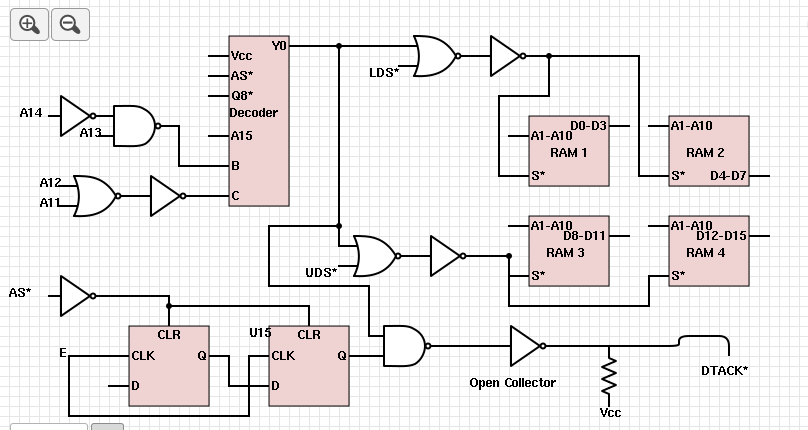
\includegraphics[width=1\linewidth]{schematic}
	\caption{Schematic for RAM Design}
	\label{fig:schematic}
\end{figure}
\begin{figure}[H]
\centering
\includegraphics[width=1\linewidth]{topdown}
\caption{Top Down View of Physical Circuit}
\label{fig:topdown}
\end{figure}

\begin{figure}[H]
\centering
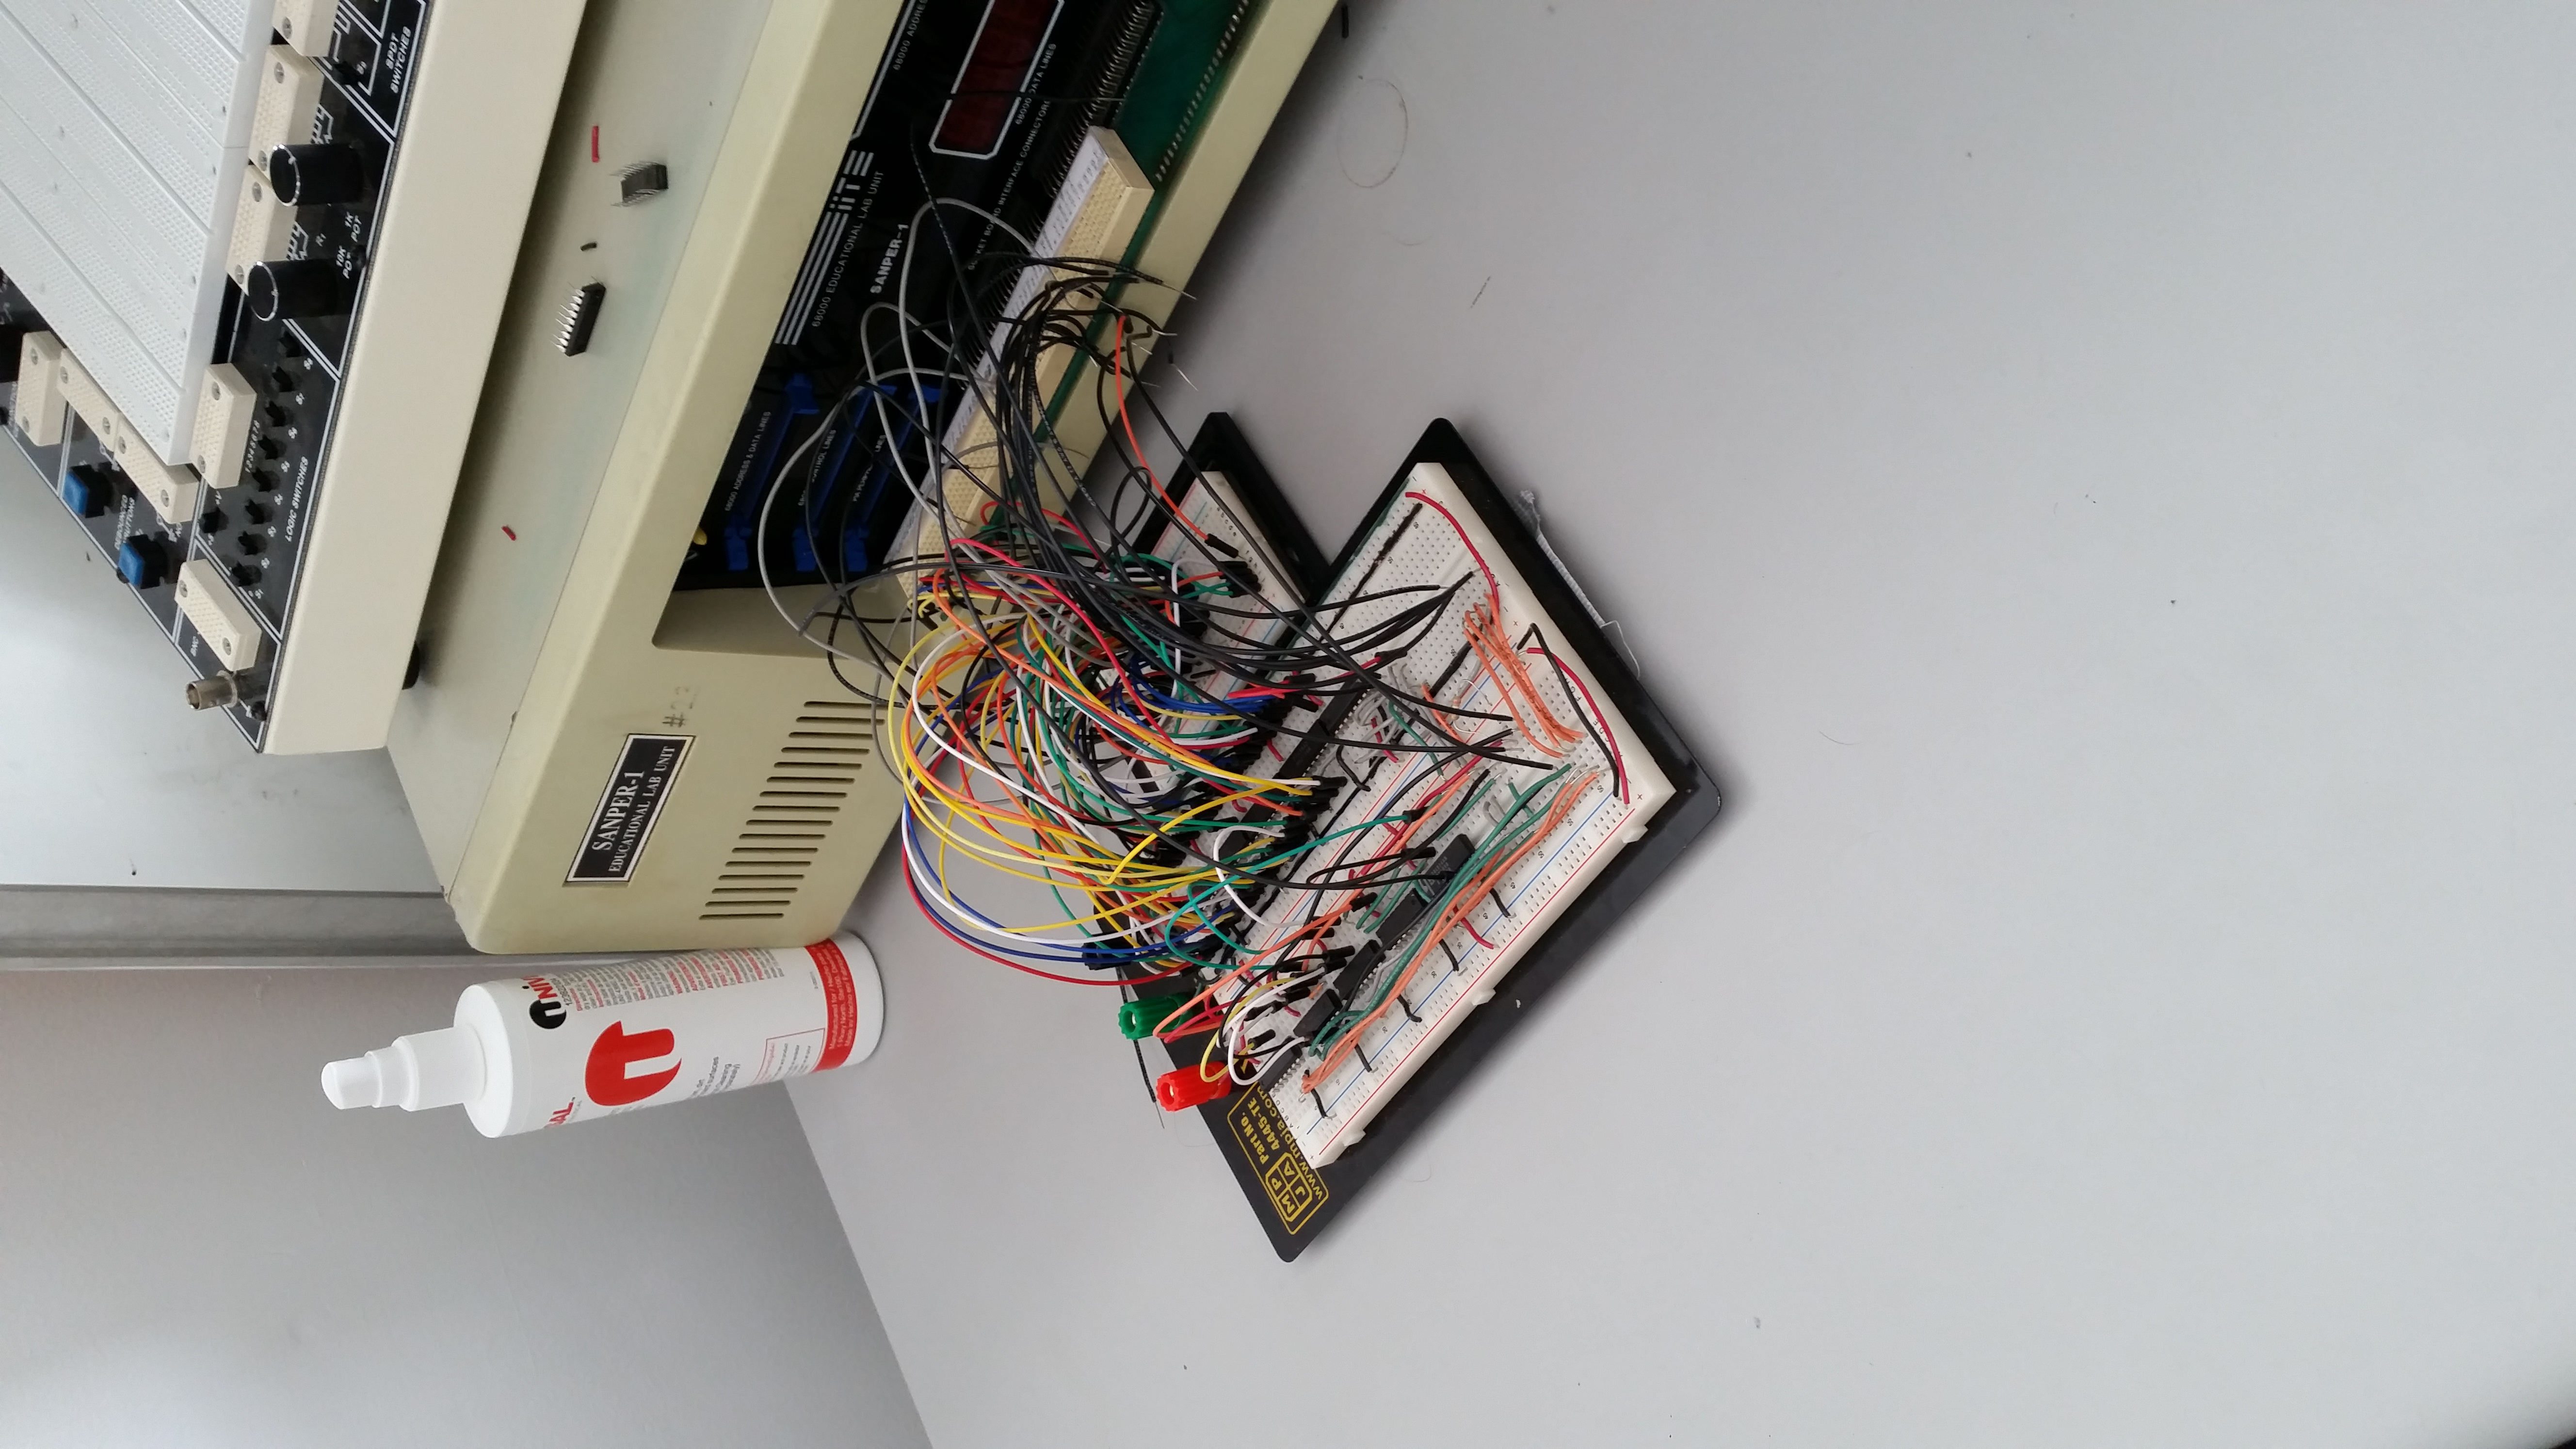
\includegraphics[width=1\linewidth]{connected}
\caption{Circuit Implementation with SANPER-1 ELU}
\label{fig:connected}
\end{figure}

\subsection{Code}\label{code}
\subsubsection{Memory Test}\label{sec:memtest}
\lstset{language=[Motorola68k]Assembler}
\lstinputlisting{RAM.X68}
\end{document}